
% This LaTeX was auto-generated from an M-file by MATLAB.
% To make changes, update the M-file and republish this document.

\documentclass{article}
\usepackage{graphicx}
\usepackage{color}
\usepackage{listings}
\usepackage[framed]{mcode}
\usepackage{fullpage}
\usepackage{amsmath}
\usepackage[utf8x]{inputenc}
\usepackage{import}
\usepackage{setspace}
\usepackage{hyperref}
\definecolor{lightgray}{gray}{0.5}
\setlength{\parindent}{0pt}

\begin{document}

    
    
%\section*{}


\title{BE 521: Homework 6 \\{\normalsize Spike sorting}\\{\normalsize Spring 2021}}
\author{60 points}
\date{Due: Tuesday, 03/09/2021 10:00pm}
\maketitle \textbf{Objective:} Detect and cluster spikes


\begin{center} \author{Jal Mahendra Panchal \\
  \normalsize Collaborators: Shreya Parchure \\}
\end{center}


\subsection*{Overview}
In this homework, you will do some basic spike sorting using two different datasets. The first (\verb|I521_A0006_D001|) is from a crayfish neuromuscular junction, a good model for human central nervous system synapses\footnote{The sampling rate of this data is 2000 Hz, which is adequate for this homework's instructional purposes but usually inadequate for real spike sorting, which often uses sampling frequencies on the order of 20 kHz.}. Specifically, the data contains two simultaneous recordings: an extracellular recording from the third nerve (channel \verb|nerve|) of a crayfish abdominal ganglion, which contains six spontaneously active motor neurons, and an intracellular recording from the superficial flexor muscle (channel \verb|muscle|) innervated by this nerve. You will attempt to discern relationships between the classes of spike waveforms you extract from the motor nerve trace and elicited potentials seen in the muscle fiber recording.
Then, you will revisit a human intracranial EEG recording (\verb|I521_A0006_D002|) and use some of the techniques you've learned in class to build a more automated spike sorter.
Note: While spikes may have positive and negative deflections, we will only focus on positive spikes on this homework for simplicity.
\section{Spike Detection and Clustering (38 pts)}
In this section, you will explore some basic filtering and spike thresholding to ultimately compare spike clusters you pick out by eye to those selected by an automated algorithm.
\begin{enumerate}
    \item You can assume that the nerve samples have already been low-pass filtered. Here you will high-pass filter in order to remove signals like slow local field potentials and 60 Hz power line noise. Create a 4th order \textit{elliptic filter} with 0.1 dB of ripple in the passband, a stopband 40 dB lower than the peak value in the passband, and a passband edge frequency of 300 Hz (see Matlab's \verb|ellip| function and make sure your give the edge frequency in the correct normalized form). The statement to create this filter (defined by the filter coefficients \verb|b| and \verb|a|) should look something like
  \begin{lstlisting}
	[b,a]=ellip(n,Rp,Rs,Wp,'high')
  \end{lstlisting}
  Clearly specify the denominator and numerator coefficients obtained for your filter function. (2pts)

$\textbf{Answer 1.1} \\$
\begin{lstlisting}
%ellip filter
n = 4 ; %4th order filter
Rp = 0.1 ; %pass band ripple in db
Rs  = 40 ; % stop band attenuation in db
Wp = 300 ; %pass band edge frequency in hz

fs = 2000; %sampling freq in hz
Wp  = Wp/fs; % converting cutoff freq to a ratio of sampling freq

[nmtr_b , den_a ] = ellip(n,Rp, Rs , Wp, 'high') ;
\end{lstlisting}
The filter's numerator and denomerator respectively are
\begin{lstlisting}
nmtr_b
den_a

figure();
freqz(nmtr_b, den_a);
title('4th order elliptic filter')
\end{lstlisting}

\color{lightgray} \begin{lstlisting}
nmtr_b =

    0.5921   -2.3307    3.4775   -2.3307    0.5921


den_a =

    1.0000   -2.9229    3.3649   -1.7764    0.3668

\end{lstlisting} \color{black}


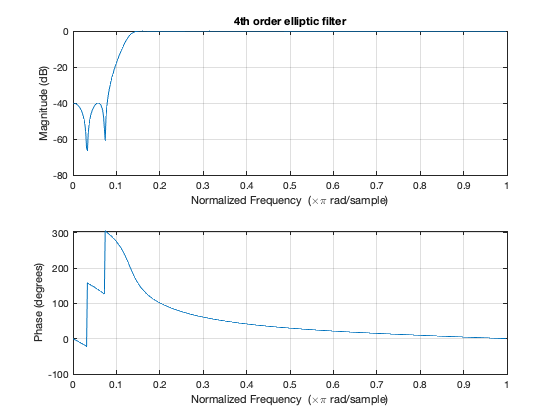
\includegraphics [width=5in]{jalp_hw6_01.png}

  \item Using the \verb|filter| function and \verb|filtfilt| function, obtain two different filtered outputs of the nerve signal.
      \begin{enumerate}
        \item In a 2x1 subplot, plot the first 50 ms of the unfiltered nerve signal in the top subplot; in the bottom subplot, plot the \verb|filter| output in blue and the \verb|filtfilt| output in red. Use a potential range (y-axis) of -20 to 50 millivolts. (4 pts)

$\textbf{Answer 1.2a} \\$
\begin{lstlisting}
%obtaining the I521_A0006_D001 signal
addpath(genpath('/Users/jalpanchal/git/be521'));

session_cray = IEEGSession('I521_A0006_D001', 'jalpanchal', 'jal_ieeglogin.bin');
sampling_frequency_hz_cray = session_cray.data.sampleRate;
duration_in_sec_cray = session_cray.data(1).rawChannels(1).get_tsdetails.getDuration/1e6;

muscle_raw_uV = session_cray.data.getvalues(0, duration_in_sec_cray * 1e6, 1);
nerve_raw_uV = session_cray.data.getvalues(0, duration_in_sec_cray * 1e6, 2);
\end{lstlisting}

\color{lightgray} \begin{lstlisting}IEEGSETUP: Adding 'ieeg-matlab.jar' to dynamic classpath
IEEGSETUP: Found log4j on Java classpath.
URL: https://www.ieeg.org/services
Client user: jalpanchal
Client password: ****
\end{lstlisting} \color{black}
\begin{lstlisting}
%filtering using filter
nerve_filter_uV = filter(nmtr_b,den_a,nerve_raw_uV);

%filtering using filtfilt
nerve_filtfilt_uV = filtfilt(nmtr_b,den_a,nerve_raw_uV);
\end{lstlisting}
\begin{lstlisting}
%plot
fs = sampling_frequency_hz_cray;
t = 0 : 1e3/sampling_frequency_hz_cray : duration_in_sec_cray*1e3 - 1e3/sampling_frequency_hz_cray ;

figure();
ax1 = subplot(2,1,1);
plot(t, nerve_raw_uV/1000, 'Linewidth', 1)
title('Nerves channel raw')
xlabel('Time (ms)')
ylabel('Signal Amplitude (mV)')
xlim([0, 50])
ylim([-20 50])

ax2 = subplot(2,1,2);
plot(t, nerve_filter_uV/1000, 'Linewidth', 1, 'color',[0 0.4470 0.7410] );
hold on
plot(t, nerve_filtfilt_uV/1000, 'Linewidth', 1, 'color', [0.6350 0.0780 0.1840]);
hold off
title('Nerves channel filtered')
xlabel('Time (ms)')
ylabel('Signal Amplitude (mV)')
legend('filter()', 'filtfilt()')
xlim([0, 50])
ylim([-20 50])

suptitle('Filtering nerve channel data for I521\_A0006\_D001')
\end{lstlisting}


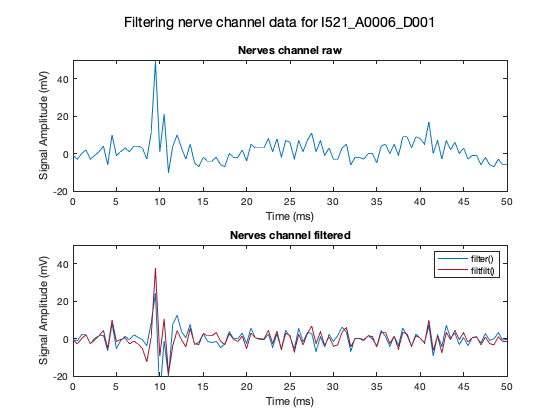
\includegraphics [width=5in]{jalp_hw6_02.png}

        \item How is the unfiltered signal different from the filtered signal? What is different about the two filtered (red and blue) signals? (2 pts)

$\textbf{Answer 1.2b} \\$
The unfiltered signal has low frequency components and a 60 Hz power line noise that can be seen as a base line fluctuation. In the filtered signals, the lower frequencies have been removed and a stable baseline can be seen. $\\$ The $filtfilt$ function processes the signal in the forward and reverse direction to cause a zero phase distortion as compared to the $filter$ function which processes the signal only in the forward direction and can result in a phase shift. The $filtfilt$ function due to its two direction approach results in doubling of the order of filter as specified by the filter coefficients b(numerator) and a(denominator). The $filter$  function in contrast maintains the order of the filter. The $filtfilt$ function does a better job of filtering low frequency signal and removing baseline fluctuations.

        \item Briefly explain the mathematical difference between the two filtering methods, and why one method might be more advantageous than the other in the context of spike detection? (5 pts)

$\textbf{Answer 1.2c} \\$
The $filter$ function in matlab uses a rational transfer function defined by the given filter coefficients b(numerator) and a(denomerator) to convert the unfiltered input signal to a filtered output signal. This process can result in a phase shift between the filtered and raw signal. This is a causal filter. $\\$ In contrast, the $filtfilt$ function is a non-causal filter that that filters the signal in the forward and reverse direction. This 2 pass method results in negating the phase shift of a single filter pass and hence results in a zero-phase distortion of the original signal. Due to the 2 pass method, the resultant transfer function is equal to the squared magnitude of the original transfer function. This also results in the doubling of the order of the effective filter as compared to the $filter$ function. $\\$ The $filtfilt$ function due to its zero-phase distortion, sharper cut-off and higher attenuation in its stop band is more suitable for spike detection as compared to $filter$ function. The phase shift could cause shift in the peak position. Also as seen from the plot above, the $filtfilt$ function does a better job of filtering low frequency signal and removing baseline fluctuations and hence is the preferred choice.

      \end{enumerate}
        \item Using a spike threshold of +30 mV, calculate the index and value of the peak voltage for each spike in the \textbf{filtered} nerve signal (select the best one). Use these values to plot the first 2.5 seconds of the nerve signal with a red dot above (e.g. 10 mV above) each spike. (Hint: Plot the entire length of the nerve signal with all the spikes marked but then restrict the x-axis using \verb|xlim| to [0, 2.5] seconds) (4 pts)

$\textbf{Answer 1.3} \\$
\begin{lstlisting}
%peak identification
x = nerve_filtfilt_uV/1000;
threshold = 30;

%finding peak using sign change in second derivative(maxima) for signal above
%threshold
peak_find = @(x, th) (find((diff(diff(x) < 0 ) .* (x(2:end-1) >th))>0));

nerve_ff_peakidx = peak_find(x,threshold);
\end{lstlisting}
\begin{lstlisting}
%plotting peaks in filtered signal
fs = sampling_frequency_hz_cray;
t = 0 : 1e3/sampling_frequency_hz_cray : duration_in_sec_cray*1e3 - 1e3/sampling_frequency_hz_cray ;
figure();
plot(t/1000, x, 'Linewidth', 1);
hold on;
plot(0 + ((nerve_ff_peakidx)/fs), x(nerve_ff_peakidx+1)+10, '.', 'Markersize',10, 'color' ,[0.8500 0.3250 0.0980] );
hold off;
ylabel('Amplitude (mV)');
xlabel('Time (sec)');
title('Nerves channel filtered (filtfilt) for I521\_A0006\_D001');
legend('filtered signal', 'peaks>30mV')
xlim([0 2.5])
\end{lstlisting}


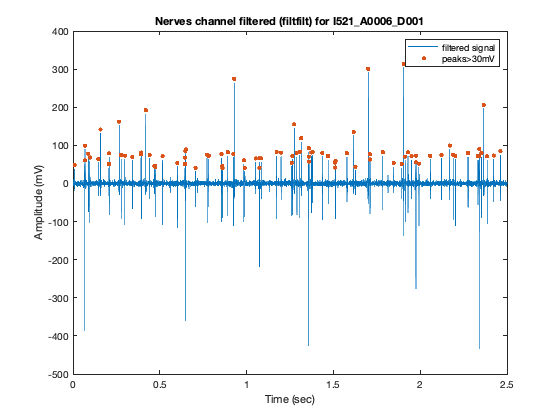
\includegraphics [width=5in]{jalp_hw6_03.png}

 \item Under the assumption that different cells produce different action potentials with distinct peak amplitudes, decide how many cells you think were recorded (some number between 1 and 6). You may find it helpful to zoom in and pan on the plot you made in question 1.3. You may also find it useful to plot the sorted peak values to gain insight into where ``plateaus'' might be. (No need to include these preliminary plots in the report, though.) Use thresholds (which you well set manually/by eye) to separate the different spikes. Make a plot of the first 2.5 seconds similar to that in 1.3 except now color the spike dots of each group a different color (e.g., \verb|'r.'|,\verb|'g.'|,\verb|'k.'|,\verb|'m.'|).(6 pts)

$\textbf{Answer 1.4} \\$
\begin{lstlisting}
nerve_peak_amp = sort(x(nerve_ff_peakidx+1));
\end{lstlisting}
Based on manual inspection of the spike amplitude and shape, it appears that 5 different neurons are recorded in the nerve channel of the signal. The first band from (30,50), second from (50,85), third from (85,155), fourth from (155,201) and the last neuron from \ensuremath{>}201 mV.
\begin{lstlisting}
%plotting peaks in filtered signal
x = nerve_filtfilt_uV/1000;
fs = sampling_frequency_hz_cray;
t = 0 : 1e3/sampling_frequency_hz_cray : duration_in_sec_cray*1e3 - 1e3/sampling_frequency_hz_cray ;

%making a cell array for each neuron peak
n = {};
n{1} = find(x(nerve_ff_peakidx+1) <50 & x(nerve_ff_peakidx+1)>=30);
n{2} = find(x(nerve_ff_peakidx+1) <85 & x(nerve_ff_peakidx+1)>=50);
n{3} = find(x(nerve_ff_peakidx+1) <155 & x(nerve_ff_peakidx+1)>=85);
n{4} = find(x(nerve_ff_peakidx+1) <201 & x(nerve_ff_peakidx+1)>=155);
n{5} = find(x(nerve_ff_peakidx+1) <310 & x(nerve_ff_peakidx+1)>=201);

figure();
plot(t/1000, x, 'Linewidth', 1);
hold on;
%plot all peaks
% plot(0 + (nerve_ff_peakidx/fs), x(nerve_ff_peakidx+1)+10, '.', 'Markersize',10, 'color' ,[0.8500 0.3250 0.0980] );

plot(nerve_ff_peakidx(n{1})/fs, x(nerve_ff_peakidx(n{1})+1) +10,'r.', 'Markersize',15);
plot(nerve_ff_peakidx(n{2})/fs, x(nerve_ff_peakidx(n{2})+1)+ 10,'b.', 'Markersize',15);
plot(nerve_ff_peakidx(n{3})/fs, x(nerve_ff_peakidx(n{3})+1)+ 10,'g.', 'Markersize',15);
plot(nerve_ff_peakidx(n{4})/fs, x(nerve_ff_peakidx(n{4})+1)+ 10,'k.', 'Markersize',15);
plot(nerve_ff_peakidx(n{5})/fs, x(nerve_ff_peakidx(n{5})+1)+ 10,'m.', 'Markersize',15);

hold off;
ylabel('Amplitude (mV)');
xlabel('Time (sec)');
title('Nerves channel manual clustering of neurons for I521\_A0006\_D001');
legend('filtered signal','neuron1', 'neuron2', 'neuron3', 'neuron4', 'neuron5')
xlim([0 2.5])
ylim([-500, 600])
\end{lstlisting}


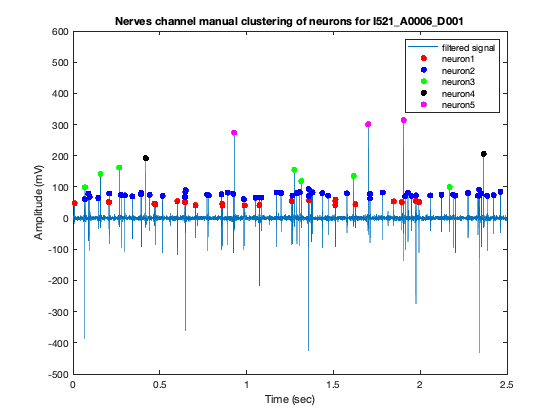
\includegraphics [width=5in]{jalp_hw6_04.png}

 \item Use Matlab's $k$-means\footnote{Clustering, like $k$-means you are using here, is a form of unsupervised learning.} function (\verb|kmeans|) to fit $k$ clusters (where $k$ is the number of cells you think the recording is picking up) to the 1D data for each spike.
  \begin{enumerate}
	\item Using the same color order (for increasing spike amplitude) as you did for the thresholds in question 1.4, plot the spike cluster colors as little dots slightly above those you made for question 1.4. The final figure should be a new plot of the nerve voltage and two dots above each spike, the first being your manual label and the second your clustered label, which (hopefully/usually) should be the same color. (4 pts)

$\textbf{Answer 1.5a} \\$
\begin{lstlisting}
%kmeans clustering
rng(1); % For reproducibility
n_clusters = 5;
[idx, centroid] = kmeans( x(nerve_ff_peakidx+1), n_clusters);
[~,i] = sort(centroid);

km_n = {};

km_n{1} = find(idx==i(1));
km_n{2} = find(idx==i(2));
km_n{3} = find(idx==i(3));
km_n{4} = find(idx==i(4));
km_n{5} = find(idx==i(5));
\end{lstlisting}
\begin{lstlisting}
%plotting clusters
figure();
plot(t/1000, x, 'Linewidth', 1);
hold on;

%plotting manaul peaks
plot(nerve_ff_peakidx(n{1})/fs, x(nerve_ff_peakidx(n{1})+1) +10,'r.', 'Markersize',10);
plot(nerve_ff_peakidx(n{2})/fs, x(nerve_ff_peakidx(n{2})+1)+ 10,'b.', 'Markersize',10);
plot(nerve_ff_peakidx(n{3})/fs, x(nerve_ff_peakidx(n{3})+1)+ 10,'g.', 'Markersize',10);
plot(nerve_ff_peakidx(n{4})/fs, x(nerve_ff_peakidx(n{4})+1)+ 10,'k.', 'Markersize',10);
plot(nerve_ff_peakidx(n{5})/fs, x(nerve_ff_peakidx(n{5})+1)+ 10,'m.', 'Markersize',10);

%plotting kmeans clusters
plot(nerve_ff_peakidx(km_n{1})/fs, x(nerve_ff_peakidx(km_n{1})+1)+30,'r.', 'Markersize',10);
plot(nerve_ff_peakidx(km_n{2})/fs, x(nerve_ff_peakidx(km_n{2})+1)+30,'b.', 'Markersize',10);
plot(nerve_ff_peakidx(km_n{3})/fs, x(nerve_ff_peakidx(km_n{3})+1)+30,'g.', 'Markersize',10);
plot(nerve_ff_peakidx(km_n{4})/fs, x(nerve_ff_peakidx(km_n{4})+1)+30,'k.', 'Markersize',10);
plot(nerve_ff_peakidx(km_n{5})/fs, x(nerve_ff_peakidx(km_n{5})+1)+30,'m.', 'Markersize',10);

hold off;
ylabel('Amplitude (mV)');
xlabel('Time (sec)');
title('Nerves channel comparing manual clustering to kmeans clustering for I521\_A0006\_D001');
legend('filtered signal', 'neuron1', 'neuron2', 'neuron3', 'neuron4', 'neuron5', 'neuron6')
xlim([0 2.5])
ylim([-500, 700])
\end{lstlisting}


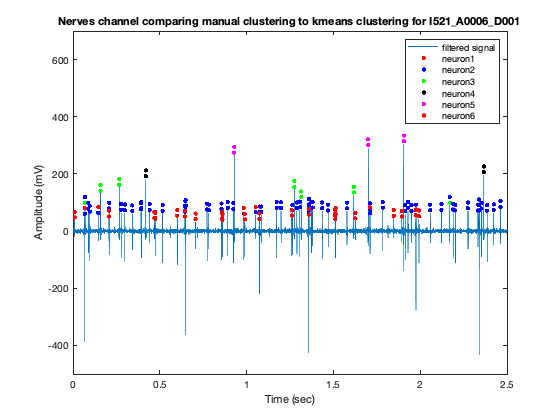
\includegraphics [width=5in]{jalp_hw6_05.png}

	\item Which labeling, your manual ones or the ones learned by clustering) seem best, or do they both seem just as good? (Again, panning over the entire plot may be helpful.) (2 pts)

$\textbf{Answer 1.5b} \\$
Based the the graph above, I would prefer the manual clustering as compared to the k-means clustering. Though the k-means clustering does a pretty good job, for peaks close to each other in time, k-means clustering seems to have clustered them in the same group though while they were in different clusters in my sorting. Also, in manual clustering I am able to see anomalies and set the threshold accordingly while k-means does not account for that. Given a very large data set, I wouldn't mind using k-means clustering as the errors average out and it might do better. But for the given data I would prefer the manual clustering method. Another aspect about the k-means clustering is the random nature of clusters when I redo clustering which is unreliable and not preferred.

  \end{enumerate}
 \item In this question,  you will test the hypothesis that the muscle potential responses are really only due to spikes from a subset of the cells you have identified in the previous two questions. First, plot the first 2.5 seconds of the muscle fiber potential and compare it with that of the nerve. Observe the relationship between spikes and the muscle fiber response. (No need to include this plot and observation in your report.)
     Now, calculate the maximum muscle fiber potential change\footnote{max voltage - min voltage} in the 25 ms\footnote{Note that this 25 ms window is somewhat ad hoc and is just what seems reasonable by eye for this data. It implies no underlying physiological time scale or standard.} window after each spike (with the assumption that spikes without any/much effect on the muscle fiber potential do not directly innervate it).
  \begin{enumerate}
   \item Using the cell groups you either manually defined or found via $k$-means clustering (just specify which you're using) again with different colors, plot a colored point for each spike where the x-value is the spike amplitude and the y-value is the muscle potential change. (6 pts)

$\textbf{Answer 1.6a} \\$
\begin{lstlisting}
%plotting peaks in filtered signal
fs = sampling_frequency_hz_cray;
t = 0 : 1e3/sampling_frequency_hz_cray : duration_in_sec_cray*1e3 - 1e3/sampling_frequency_hz_cray ;
figure();
yyaxis left
plot(t/1000, x, 'Linewidth', 1);
ylabel('Amplitude (mV)');
hold on;

yyaxis right
plot(t/1000, muscle_raw_uV/1000,  'color' ,[0.8500 0.3250 0.0980] );
ylabel('Amplitude (mV)');
ylim([-76, -50])

%plotting markers for peaks
% for i = 1:size(nerve_ff_peakidx/fs,1)
%         xline(nerve_ff_peakidx(i)/fs);
% end

hold off;

xlabel('Time (sec)');
title('nerve and muscle channel for I521\_A0006\_D001');
legend('filtered nerve signal', 'muscle channel')
xlim([0 2.5])
\end{lstlisting}


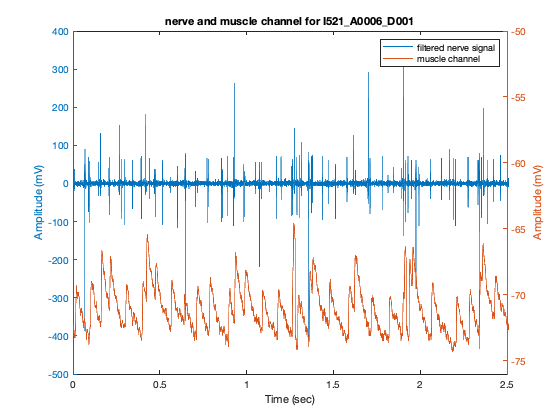
\includegraphics [width=5in]{jalp_hw6_06.png}
Using manual clustering to sort cell groups for analysing muscle potential responses
\begin{lstlisting}
%calculating muscle fiber potential change after neuron spike
pot_change_peak = {};
%first we loop through the different sets of neuron clusters
for i= 1:n_clusters
    idx = n{i};
    temp_ = zeros(size(idx,1),3);
    for j = 1:size(idx,1)
       %calculating max and min mulscle voltage in 25 ms window after peak
       window_ms = 25;
       samples = window_ms*fs/1000;
       %index of signal of peak #j in neuron cluster i
       pk_idx = nerve_ff_peakidx(idx(j))+1;
       muscle_sig = muscle_raw_uV(pk_idx : pk_idx+samples);
       muscle_pot_mV = (max(muscle_sig)-min(muscle_sig))/1000;

       %saving, peak index, muscle pot change and spike amplitude in matrix
       temp_(j,:) = [pk_idx-1, muscle_pot_mV,x(pk_idx)];
    end
    %cell array of temp_ matrix for each cluster
    pot_change_peak{i} = temp_;
end
\end{lstlisting}
\begin{lstlisting}
%plotting peaks in filtered signal
fs = sampling_frequency_hz_cray;
t = 0 : 1e3/sampling_frequency_hz_cray : duration_in_sec_cray*1e3 - 1e3/sampling_frequency_hz_cray ;
figure();

plot(pot_change_peak{1}(:,3), pot_change_peak{1}(:,2),'r.', 'Markersize',15);
hold on
plot(pot_change_peak{2}(:,3), pot_change_peak{2}(:,2),'b.', 'Markersize',15);
plot(pot_change_peak{3}(:,3), pot_change_peak{3}(:,2),'g.', 'Markersize',15);
plot(pot_change_peak{4}(:,3), pot_change_peak{4}(:,2),'k.', 'Markersize',15);
plot(pot_change_peak{5}(:,3), pot_change_peak{5}(:,2),'m.', 'Markersize',15);
hold off;

ylabel('Potential Change(mV)');
xlabel('Peak Amplitude(mV)');
title('Spike peak amplitude vs Muscle potential change, manual clusters  I521\_A0006\_D001');
legend('neuron1', 'neuron2', 'neuron3', 'neuron4', 'neuron5')
% xlim([0 2.5])
\end{lstlisting}


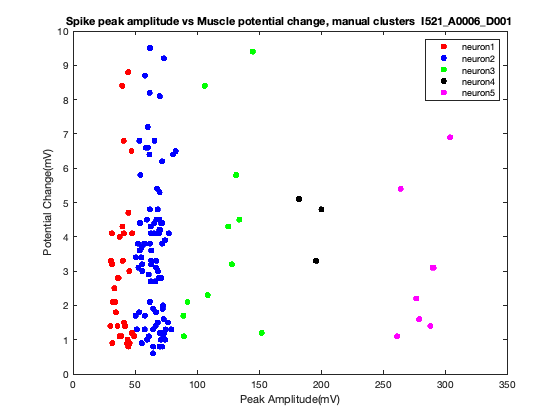
\includegraphics [width=5in]{jalp_hw6_07.png}

   \item Does this plot support the hypothesis that the muscle fiber responses are only due to a subset of the cells. Explain why or why not. (3 pts)

$\textbf{Answer 1.6b} \\$
In the Spike peak amplitude vs muscle potential change plot, we don't quite see a relation between muscle potential response and spike clusters or spike amplitude. The number of spikes in each cluster is not the same so it it hard to make a conclusion. What we do see is that for neuron with lower peak spike amplitude there seems to be higher potential change, this could be due to the fact that these spikes often appear in sets. For neurons with higher spike amplitude the potential change seems to be smaller. Though no cluster - potential change conclusion can be drawn from this data and due to the low number of data points in clusters. So we cannot support the hypothesis that muscle fiber responses are only due to a subset of the cells from this data and plot.

  \end{enumerate}
\end{enumerate}
\section{Multivariate Clustering (22 pts)}
In this section, you will explore similar methods for spikes sorting and clustering but with a different dataset, the human intracranial data in \verb|I521_A0006_D002|,
which is a larger dataset of the same recording you saw in \verb|I521_A0001_D001| of Homework 1.
  \begin{enumerate}
   \item Using a threshold six standard deviations above the mean of the signal, detect the spikes in the signal. In addition, extract the waveform from 1 ms before the peak to 1 ms after it with peak value in the middle. (You will end up with a matrix where each row corresponds to the number of data points in 2 ms of signal minus 1 data point. Use the closest integer number of data points for the $\pm$ 1 ms window.)


	\begin{enumerate}
	  \item Plot the waveforms of all the spikes overlaid on each other in the same color. (4 pts)

$\textbf{Answer 2.1a} \\$
\begin{lstlisting}
%obtaining the I521_A0006_D002 signal
addpath(genpath('/Users/jalpanchal/git/be521'));

session_humn = IEEGSession('I521_A0006_D002', 'jalpanchal', 'jal_ieeglogin.bin');
sampling_frequency_hz_humn = session_humn.data.sampleRate;
duration_in_sec_humn = session_humn.data(1).rawChannels(1).get_tsdetails.getDuration/1e6;

intcran_raw_uV = session_humn.data.getvalues(0, duration_in_sec_humn * 1e6, 1);
\end{lstlisting}

\color{lightgray} \begin{lstlisting}IEEGSETUP: Adding 'ieeg-matlab.jar' to dynamic classpath
Warning: Objects of edu/upenn/cis/db/mefview/services/TimeSeriesDetails class
exist - not clearing java 
Warning: Objects of edu/upenn/cis/db/mefview/services/TimeSeriesInterface class
exist - not clearing java 
IEEGSETUP: Found log4j on Java classpath.
URL: https://www.ieeg.org/services
Client user: jalpanchal
Client password: ****
\end{lstlisting} \color{black}
\begin{lstlisting}
%calculating peaks above 6 std above mean

std_humn_uV = std(intcran_raw_uV);
mean_humn_uV = mean(intcran_raw_uV);

threshold_uV = mean_humn_uV + 6*std_humn_uV;

humn_peak_idx = peak_find(intcran_raw_uV, threshold_uV);
\end{lstlisting}
\begin{lstlisting}
%plotting human intercranial signal raw
fs = sampling_frequency_hz_humn;
t = 0 : 1/fs : duration_in_sec_humn;
x = intcran_raw_uV;
figure();
plot(t, x, 'Linewidth', 1);
hold on
yline(threshold_uV, '-','threshold');
plot(0 + ((humn_peak_idx)/fs), x(humn_peak_idx+1)+1, '.', 'Markersize',10, 'color' ,[0.8500 0.3250 0.0980] );
hold off;
ylabel('Signal Amplitude (\muV)');
xlabel('Time (sec)');
title('Intracranial human data for I521\_A0006\_D002');
\end{lstlisting}


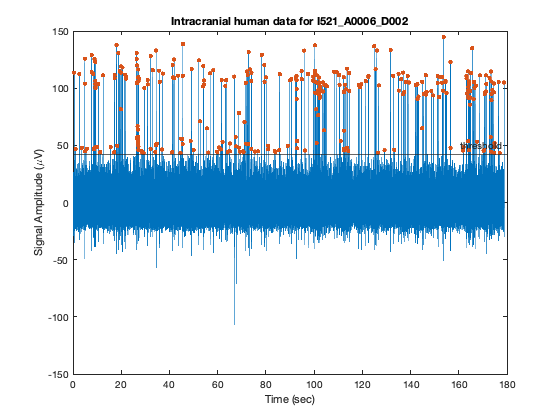
\includegraphics [width=5in]{jalp_hw6_08.png}
\begin{lstlisting}
%stacking ±1 ms around all peaks
%for a sampling frequency of 32258, 1ms has 32.258 points
% to acquire 1 ms before and after the peak, we can acquire 32 points before
% and 32 points after the peak
peak_stack_uV = zeros(size(humn_peak_idx,1), 65);
for i = 1:size(humn_peak_idx,1)
    pk_idx = humn_peak_idx(i)+1;
   peak_stack_uV(i, :) = intcran_raw_uV(pk_idx-32 : pk_idx+32);
end
\end{lstlisting}
Plotting stacked peaks
\begin{lstlisting}
t = (-32:1:32)/32258;

figure();
plot(t,peak_stack_uV(1:size(humn_peak_idx,1),:), 'color', [0 0.4470 0.7410])

xline(0)
ylabel('Signal Amplitude(\muV)');
xlabel('Time around peak (ms)');
title('Stacking aligned peaks above threshold for I521\_A0006\_D002');
\end{lstlisting}


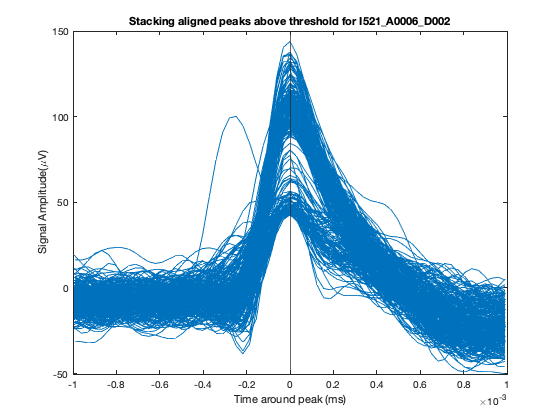
\includegraphics [width=5in]{jalp_hw6_09.png}

	  \item Does it looks like there is more than one type of spike? (1 pt)

$\textbf{Answer 2.1b} \\$
Yes, based on the stacked plots we see that there are at least 2 "groups" of peaks stacked together, one with a peak amplitude close to 50 \$\ensuremath{\backslash}mu\$V and another with a peak amplitude of about 100 \$\ensuremath{\backslash}mu\$V. This means that there are at least 2 types of spikes.There are some peaks/spikes at a higher amplitude around 125 \$\ensuremath{\backslash}mu\$V which could be another type of spike/peak.

	\end{enumerate}
   \item For each spike, represent the waveform by its  principal components. Use the \verb|pca| command in Matlab. Intuitively, principal component analysis finds the coordinate system that most reduces the variability in your data.
	\begin{enumerate}
	  \item Run principal component analysis on all the spike waveforms and represent your data with the top two principal components. Make a scatterplot of your data in this principal component (PC) space. (3 pts)

$\textbf{Answer 2.2a} \\$
\begin{lstlisting}
%performing pca analysis
humn_peak_amp_uV = peak_stack_uV(:,33);
[coeff,score,latent,tsquared,explained,mu] = pca(peak_stack_uV);
\end{lstlisting}
\begin{lstlisting}
%plotting a scatter plot in PC space
figure();
scatter(score(:,1), score(:,2), 'filled')
ylabel('Principle component 2');
xlabel('Principle component 1');
title('PC1 vs PC2, I521\_A0006\_D002 data in Principle component space');
\end{lstlisting}


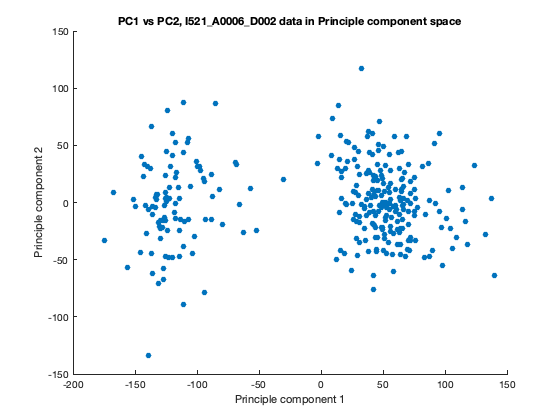
\includegraphics [width=5in]{jalp_hw6_10.png}

	  \item Each PC also has an associated eigenvalue, representing the amount of variance explained by that PC. This an output of the \verb|PCA| command. Plot the  principal component vs the total (cumulative) percent variance explained. What is the percent variance explained if you include the top two principal components? (3 pts)

$\textbf{Answer 2.2b} \\$
\begin{lstlisting}
%plotting variance for each principle component
figure();
plot(explained, 'Linewidth', 2);
ylabel('Percentage variance (%)');
xlabel('Principle component number');
title('Principle component vs percentage variance in I521\_A0006\_D002');
\end{lstlisting}


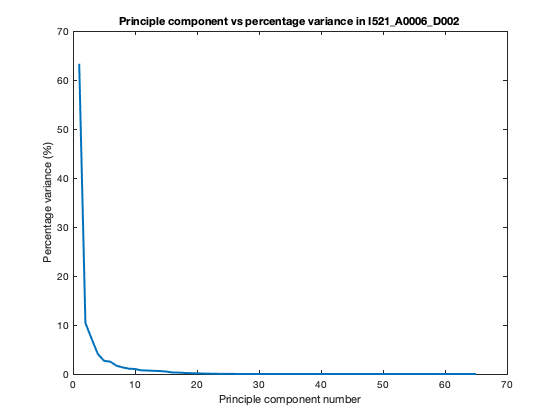
\includegraphics [width=5in]{jalp_hw6_11.png}
\begin{lstlisting}
%variance by first 2 PCs
pc12_percentage_variance  = explained(1)+explained(2)
\end{lstlisting}

\color{lightgray} \begin{lstlisting}
pc12_percentage_variance =

   73.7349

\end{lstlisting} \color{black}
The top 2 principle components explain a variance of 73.73\%

	  \item Does it look like there is more than one cluster of spikes? (1 pt)
	\end{enumerate}

$\textbf{Answer 2.2c} \\$
Yes, From the PC1 vs PC2 scatter plot above, it looks like there are 2 clusters of spikes.

   \item Use the same \verb|kmeans| function as you used before to cluster the spikes based on these two (normalized) features (the waveforms represented by the top two PCs). You will use a slight twist, though, in that you will perform $k$-medians (which uses the medians instead of the mean for the cluster centers) by using the \verb|'cityblock'| distance metric (instead of the default \verb|'sqEuclidean'| distance). Make a plot similar to that in 2.2.a but now coloring the two clusters red and green. (3 pts)

$\textbf{Answer 2.3} \\$
\begin{lstlisting}
%normalizing the vales in the PC space
score_norm = normalize(score);

%kmedians clusturing on normalized data in PC space
[idx, centroid] = kmeans( score_norm(:,1:2), 2, 'Distance', 'cityblock');
[~, i] = sort(centroid);
km_pc_idx = {};

km_pc_idx{1} = find(idx==i(1));
km_pc_idx{2} = find(idx==i(2));
\end{lstlisting}
\begin{lstlisting}
%scatter plot for clusters
figure();
scatter(score_norm(km_pc_idx{1},1), score_norm(km_pc_idx{1},2), 'filled','MarkerfaceColor', [0.6350 0.0780 0.1840])
hold on
scatter(score_norm(km_pc_idx{2},1), score_norm(km_pc_idx{2},2), 'filled', 'MarkerfaceColor', [0.4660 0.6740 0.1880])
hold off
ylabel('Principle component 2');
xlabel('Principle component 1');
title('PC1 vs PC2, 2 clusters: k-medians for I521\_A0006\_D002');
\end{lstlisting}


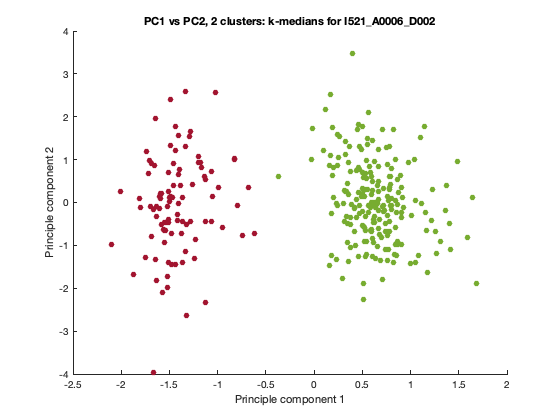
\includegraphics [width=5in]{jalp_hw6_12.png}

  \item Make a plot similar to 2.1 but now coloring the traces red and green according to which cluster they are in. Overlay the mean of the waveforms in each cluster with a thick black line (use the parameter \verb|'LineWidth'| and value \verb|'4'|). (3 pts)

$\textbf{Answer 2.4} \\$
\begin{lstlisting}
%plotting clustered stacks of peaks
t = (-32:1:32)/32258;

figure();
%cluster 2 stacks
plot(t,peak_stack_uV(km_pc_idx{2},:), 'color', [0.4660 0.6740 0.1880])
hold on
%plotting mean for cluster 2
plot(t, mean(peak_stack_uV(km_pc_idx{2},:)), 'Linewidth', 4, 'color', 'k')

%cluster 1 stacks
plot(t,peak_stack_uV(km_pc_idx{1},:), 'color', [0.6350 0.0780 0.1840])
%plotting mean for cluster 1
plot(t, mean(peak_stack_uV(km_pc_idx{1},:)), 'Linewidth', 4, 'color', 'k')

xline(0)
ylabel('Signal Amplitude(\muV)');
xlabel('Time around peak (ms)');
title('Stacking aligned peaks showing 2 clusters for I521\_A0006\_D002');
\end{lstlisting}


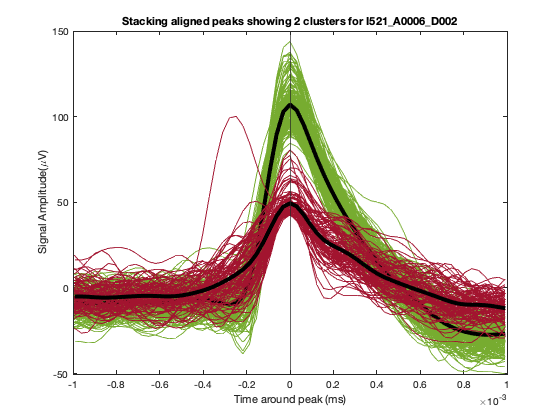
\includegraphics [width=5in]{jalp_hw6_13.png}

  \item What is a disadvantage of using principal component analysis? (1 pts)

$\textbf{Answer 2.5} \\$
The biggest disadvantage of PCA is interpretation of the principle components. We don't know what the principle components actually are and what they represent with respect to the data. If we want to understand the physiological importance of features/components, this will not be possible from the principle components as they are mathematical constructs.

  \item What are some dangers of using the clustering techniques in this homework? (List 3) (3 pts)

$\textbf{Answer 2.6} \\$

Some of the dangers of the clustering techniques are:
\begin{enumerate}
\item The k-means clustering relied on the number of clusters fed by me.
This is a big drawback as I must analyse the data enough to identify the
number of clusters, specially difficult if the borders are very close. If I choose
the wrong numbers of clusters it will impact the operations down the processing line.
\item Another challenge with the k-means function in Matlab was the random
nature of iterations it computes. Due to the random initialization, I
found the clusters to be different at times which leads to non reliable
results. Its hard to assess what is the right seed to initialize the
function for optimal clustering.
\item The clusters also had hard thresholds which made the sorting of
points close to the border a challenge. This also gets worse if the
algorithm reaches a local minima due to its random initialization.
\end{enumerate}


\end{enumerate}
\end{document}




\end{document}
    
